\chapter{Desenvolvimento da Solução}\label{chp:dev}

Este capítulo descreve como a solução foi construída: o ambiente de desenvolvimento, a organização do repositório, a evolução por incrementos, o acompanhamento com a orientação, o registro das decisões e a manutenção da documentação. As informações sobre a evolução do código foram extraídas do histórico de versionamento, de modo que cada afirmação sobre o processo pode ser conferida por um identificador de \textit{commit}.

\section{Preparação do Ambiente}
\label{sec:dev_ambiente}

A Tabela~\ref{tab:ambiente} resume as tecnologias e ferramentas utilizadas. O ambiente foi mantido deliberadamente enxuto: o produto é um binário único, e a compilação depende apenas do compilador da linguagem e de duas bibliotecas diretas de domínio (proxy e interface de terminal), além de uma biblioteca de leitura de YAML.

\begin{table}[htb]
\centering
\caption{Ambiente e ferramentas de desenvolvimento}\label{tab:ambiente}
\small
\begin{tabular}{|p{3.6cm}|p{10.3cm}|}
\hline
\textbf{Item} & \textbf{Descrição} \\ \hline
Linguagem & Go (módulo declarado para a versão 1.25). Escolhida por gerar binário único multiplataforma, por oferecer biblioteca padrão para HTTP, TLS e certificados X.509. \\ \hline
Bibliotecas & Biblioteca de proxy HTTP com suporte a interceptação TLS (\textit{goproxy}, v1.8.3); leitura e escrita de YAML (\textit{yaml.v3}, v3.0.1); interface de terminal (\textit{Bubble Tea} v1.3.10 e \textit{Lip Gloss} v1.1.0). \\ \hline
Automação local & \textit{Makefile} com alvos de compilação por plataforma, execução, diagnóstico, geração de \textit{checksums}, desinstalação da CA, testes, cobertura e \textit{benchmarks}. \\ \hline
Controle de versão & Git, com repositório público no GitHub. \\ \hline
Integração contínua & \textit{Workflow} do GitHub Actions acionado por \textit{tags} de versão, com matriz de compilação para macOS (Apple Silicon e Intel), Linux (amd64) e Windows (amd64), \textit{CGO} desabilitado, geração de \textit{checksums} SHA-256 e publicação da \textit{release}. \\ \hline
Distribuição & Binários de \textit{release}; instalação por Homebrew (macOS e Linux); \textit{script} PowerShell (Windows). \\ \hline
Dados de teste & Arquivos com credenciais fictícias, no formato dos \textit{tokens} reais mas sem validade, usados exclusivamente para testar a detecção. \\ \hline
\end{tabular}
\fonte{Elaborado pelo equipe (2026), a partir dos arquivos de configuração do repositório.}
\end{table}

\section{Organização do Repositório}
\label{sec:dev_repo}

O repositório adota uma estrutura convencional para projetos em Go, com o ponto de entrada em \texttt{cmd/} e o código de domínio em \texttt{internal/}, o que impede sua importação por outros módulos e reforça os limites entre pacotes.

\begin{lstlisting}[basicstyle=\ttfamily\scriptsize, frame=single, caption={Estrutura do repositório (simplificada)}, label={lst:repo}, captionpos=t, breaklines=true]
.
|-- cmd/<aplicacao>/main.go    # ponto de entrada: subcomandos, flags, orquestracao
|-- internal/
|   |-- ca/                    # geracao da CA local e instalacao no macOS
|   |-- guardian/              # nucleo: proxy MITM, filtro, provedor, analisador,
|   |                          #   configuracao, auditoria, instalacao de CA (Linux/Windows)
|   |-- doctor/                # diagnostico do ambiente
|   `-- tui/                   # interface de terminal (Bubble Tea)
|-- scripts/                   # scripts de conveniencia para iniciar ferramentas com proxy
|-- markdown/                  # documentacao complementar (esquema de auditoria, testes)
|-- .github/workflows/         # integracao continua e publicacao de releases
|-- Makefile, go.mod, go.sum
|-- config.yml.example         # exemplo comentado de configuracao
`-- readme.md, SECURITY.md, CONTRIBUTING.md, LICENSE
\end{lstlisting}

\textbf{Convenções.} As mensagens de \textit{commit} seguem, na maior parte do histórico, prefixos que indicam o tipo de alteração (\textit{feat}, \textit{fix}, \textit{doc}, \textit{test}, \textit{ci}, \textit{refact}). O guia de contribuição estabelece dois ramos de longa duração, um estável e um de desenvolvimento, com \textit{pull requests} de funcionalidades dirigidos a este último, além de exigir testes para novas funcionalidades e execução de \textit{benchmarks} quando o analisador ou o núcleo forem alterados. O repositório contém ainda política de segurança (relato de vulnerabilidades) e licença Apache~2.0. Arquivos de certificado, binários, \textit{checksums} e registros de auditoria são excluídos do versionamento.

\textbf{Dimensão.} O código-fonte contém cerca de 3.600 linhas de Go de produção e 1.300 linhas de testes, distribuídas em quatro pacotes internos.

\section{Implementação por Incrementos}
\label{sec:dev_incrementos}

O desenvolvimento seguiu um processo iterativo e incremental, sem \textit{sprints} formais. O histórico reúne 64 \textit{commits}, de 16 de abril a 17 de julho de 2026. A Tabela~\ref{tab:incrementos} agrupa esses \textit{commits} em nove incrementos, definidos por coesão de objetivo, e a Figura~\ref{fig:commits} mostra a distribuição semanal.

\begin{figure}[htb]
\centering
\caption{Atividade de desenvolvimento por semana}\label{fig:commits}
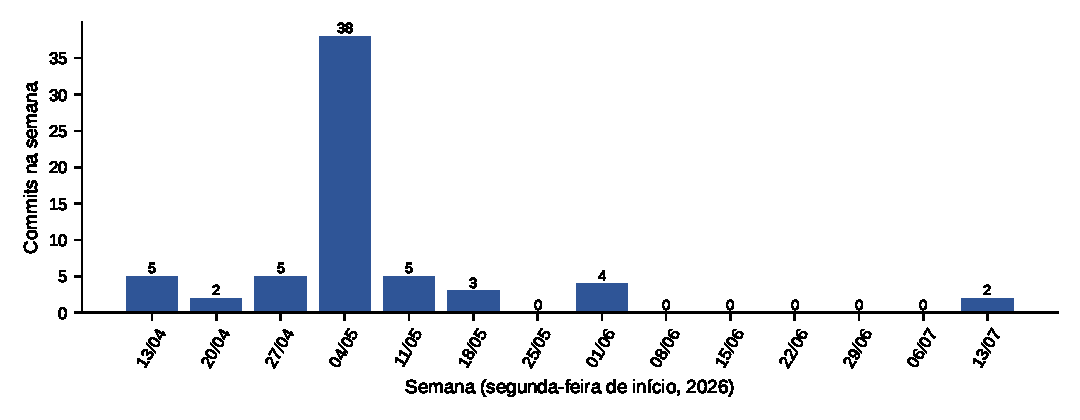
\includegraphics[width=0.9\textwidth]{figuras/commits_semana.pdf}
\fonte{Elaborado pela equipe (2026), a partir do histórico de \textit{commits}.}
\end{figure}

{\small
\begin{longtable}{|p{0.9cm}|p{2.1cm}|p{6.6cm}|p{2.6cm}|p{1.6cm}|}
\caption{Incrementos de desenvolvimento}\label{tab:incrementos}\\
\hline
\textbf{Inc.} & \textbf{Período} & \textbf{Objetivo e entregas} & \textbf{Evidência (\textit{commits})} & \textbf{Requisitos} \\ \hline
\endfirsthead
\hline
\textbf{Inc.} & \textbf{Período} & \textbf{Objetivo e entregas} & \textbf{Evidência (\textit{commits})} & \textbf{Requisitos} \\ \hline
\endhead
I0 & 16--21/04 (7 \textit{commits}) & \textbf{Exploração.} Protótipo de monitoramento TCP/HTTP, captura de tráfego em arquivo de pacotes com relatório em \textit{script} Python e tentativa de configuração por regras de \textit{firewall}. Primeira versão do analisador. & 743885b, d47a2d8, 1236bda, 6cebe4b, 2d8a085, 4de235e & --- \\ \hline
I1 & 29--30/04 (3) & \textbf{Primeira versão funcional.} Analisador por expressões regulares, registro de auditoria em arquivo, métricas e primeira documentação. Remoção do protótipo de captura de pacotes. & 8523640, 913d304, 7a7a1f1 & RF10, RF13, RF15 \\ \hline
I2 & 01--03/05 (2) & \textbf{CA local e configuração.} Geração da CA e instalação no macOS; leitura de configuração YAML com padrões personalizados e primeiro filtro de requisições. & 3683963, bdb96f0 & RF02, RF03, RF12, RF17 \\ \hline
I3 & 04/05 (9) & \textbf{Unificação e infraestrutura.} Consolidação do repositório; \textit{Makefile}; instaladores de CA para Linux e Windows; licença; \textit{workflow} de publicação; especificação do certificado. & 3fc3d71, 9317162, 93ab52a, c23afe3, 3964fb7 & RF03, RF24 \\ \hline
I4 & 05/05 (6) & \textbf{Testes de desempenho e de padrões.} \textit{Benchmark}, testes de latência e de vazão, testes de padrões personalizados e ajustes do exemplo de configuração. & ef79c09, 5bd4a00, 2d9942e, 18832a7, 7b154ff & RNF01, RNF03 \\ \hline
I5 & 06--08/05 (23) & \textbf{Integração, endurecimento e documentação.} Integração com uma segunda ferramenta de linha de comando; política de segurança e guia de contribuição; arquivo de proxy personalizado; instalação automática da CA no Linux; diagnóstico; comandos \textit{make}; desinstalação da CA; modo \textit{dry-run}; seção de riscos de segurança. & f629dd8, cd10441, 6f77577, d2c13a7, ea07ba6, 2be8767, 81de42e, aee374a, f3b3051 & RF03, RF14, RF21, RF22 \\ \hline
I6 & 12--18/05 (8) & \textbf{Refatoração do proxy.} Identificação de requisições de IA pelo corpo, inferência de provedor, modos \textit{whitelist} e \textit{passive}, limite de corpo e 370 linhas de testes de filtro; correções de CI; ajustes de documentação e demonstração. & 6a234ce, bb9872f, 8ad5a6e, 98dfe25 & RF05--RF09 \\ \hline
I7 & 02--03/06 (4) & \textbf{Interface de linha de comando e TUI.} Subcomandos e \textit{flags}; painel em tempo real; edição de padrões e do proxy com persistência no YAML; \textit{script} de instalação para Windows; pré-lançamento. & 0982721, 72e0282, 925bbc4, 0a1158e & RF18--RF20, RF24 \\ \hline
I8 & 17/07 (2) & \textbf{Distribuição e limpeza.} Documentação da instalação por Homebrew e remoção de arquivos sem uso. & 137478e, faebae9 & RF24 \\ \hline
\end{longtable}
}
\noindent\fonte{Elaborado pela equipe (2026), a partir do histórico de versionamento.}

Três observações caracterizam o processo. Primeiro, o incremento I0 foi um \textit{spike} exploratório cuja principal contribuição foi negativa: a captura passiva de pacotes não permite inspecionar o conteúdo de tráfego TLS, o que motivou a adoção do proxy com terminação TLS (decisão D01, Seção~\ref{sec:dev_decisoes}). Segundo, houve uma concentração de esforço em 4--8 de maio (38 dos 64 \textit{commits}), com predominância de infraestrutura e documentação. Terceiro, os requisitos centrais (RF10 a RF13) foram entregues cedo (I1), e os incrementos seguintes ampliaram a abrangência (I6), a operacionalidade (I3, I5) e a usabilidade (I7), o que é coerente com a priorização MoSCoW do Capítulo~\ref{chp:req}.

\section{Reuniões de Acompanhamento}
\label{sec:dev_reunioes}

O acompanhamento com a orientação é registrado em formato de ata resumida, com data, pauta, deliberações e encaminhamentos. A Tabela~\ref{tab:reunioes} reúne as orientações recebidas que já foram incorporadas ao trabalho e reserva linhas para as demais reuniões.

\begin{table}[htb]
\centering
\caption{Registro de reuniões de acompanhamento e orientações incorporadas}\label{tab:reunioes}
\small
\begin{tabular}{|p{1.8cm}|p{3.3cm}|p{5.2cm}|p{3.6cm}|}
\hline
\textbf{Data} & \textbf{Pauta} & \textbf{Deliberação / orientação} & \textbf{Encaminhamento} \\ \hline
\ 27/08/2026 & Critérios da revisão da literatura & Todas as referências devem possuir DOI ou ISSN; excluir TCCs e documentos sem revisão por pares. & Aplicado à seleção e ao arquivo de referências (Capítulo~\ref{chp:fund}). \\ \hline
\ 27/08/2026 & Justificativa do problema & Fundamentar o trabalho com casos reais de vazamento de dados. & Casos incluídos no Capítulo~\ref{chp:fund}; ampliar com fontes revisadas por pares. \\ \hline
\ 27/08/2026 & Apresentação da solução & Não nomear o produto antes do capítulo de resultados. & Texto dos Capítulos~\ref{chp:req} a~\ref{chp:test} usa descrição genérica. \\ \hline

\end{tabular}
\fonte{Elaborado pela equipe (2026).}
\end{table}


\section{Registro das Decisões}
\label{sec:dev_decisoes}

As decisões técnicas relevantes são registradas no formato de \textit{architecture decision records} simplificados: contexto e decisão, alternativas e justificativa, e consequências. Cada decisão aponta para o \textit{commit} em que se tornou observável no código. As justificativas foram reconstruídas a partir do código, do histórico e da documentação do projeto.



{\small
\begin{longtable}{|p{1.0cm}|p{4.2cm}|p{5.4cm}|p{3.3cm}|}
\caption{Registro de decisões técnicas}\label{tab:adr}\\
\hline
\textbf{ID} & \textbf{Decisão} & \textbf{Alternativas e justificativa} & \textbf{Consequências} \\ \hline
\endfirsthead
\hline
\textbf{ID} & \textbf{Decisão} & \textbf{Alternativas e justificativa} & \textbf{Consequências} \\ \hline
\endhead
D01  & Interceptar o tráfego por proxy com terminação TLS, em vez de captura passiva de pacotes ou regras de \textit{firewall}. & A captura passiva (testada em I0) observa apenas tráfego cifrado e não permite ler nem alterar o corpo; regras de \textit{firewall} só permitem bloquear. O proxy com terminação TLS é a única das alternativas que permite detectar e redigir o conteúdo. & Exige instalar e confiar numa CA local (D04) e não funciona com clientes que fixam certificados. \\ \hline
D02  & Implementar em Go. & Alternativas: linguagens com máquina virtual ou interpretadas. Go entrega binário estático multiplataforma, com biblioteca padrão para HTTP, TLS e X.509. & Distribuição simples (RNF07); dependência de biblioteca de proxy de terceiros. \\ \hline
D03  & Detectar dados sensíveis por expressões regulares e valores literais, sem classificadores de aprendizado de máquina. & Os trabalhos revisados usam modelos para reduzir falsos positivos em artefatos estáticos \cite{rahman2025secret,tsebak2025enhancing}; no caminho crítico de cada requisição, a abordagem determinística tem custo previsível, sem dependências nem inferência, e é auditável. & Cobertura limitada aos formatos conhecidos ou configurados; a evolução natural é um estágio híbrido, como o proposto nesses trabalhos. \\ \hline
D04  & Gerar uma CA exclusiva na máquina do usuário (RSA 4096, 10 anos), instalá-la no repositório do sistema e nunca versioná-la. & Alternativas: CA compartilhada distribuída com o produto (rejeitada: a chave comprometida afetaria todos os usuários) ou desativar a verificação de certificados nos clientes (rejeitada: reduz a segurança). & O usuário concede confiança à CA; a chave local torna-se ativo crítico (RNF04). \\ \hline
D05  & Configuração por arquivo YAML opcional, com padrões embutidos ativos por omissão. & Alternativas: \textit{flags} apenas ou banco de dados. O YAML é legível, versionável e editável por humanos; o funcionamento sem arquivo reduz a barreira de adoção. & Sem recarga a quente: mudanças valem na próxima inicialização. \\ \hline
D06  & Persistir a auditoria em arquivo JSON Lines, sem SGBD. & Alternativas: banco embarcado ou servidor. O arquivo de inclusão atende ao requisito de binário único e é consumível por ferramentas externas (Seção~\ref{sec:proj_dados}). & Consultas analíticas exigem ferramentas externas; proposta relacional na Seção~\ref{sec:proj_relacional}. \\ \hline
D07  & Identificar requisições de IA pelo conteúdo do corpo, e oferecer os modos \textit{whitelist} e \textit{passive}. & Alternativa: lista fixa de \textit{hosts} dos provedores (rejeitada: não cobre novas ferramentas e provedores). A identificação por corpo sustenta o agnosticismo (RNF11); o modo \textit{whitelist} reduz o escopo quando se conhecem os destinos. & Possibilidade de falsos positivos de classificação em corpos JSON com campos homônimos. \\ \hline
D08 & Oferecer modo \textit{dry-run}. & Permite validar padrões e calibrar a seletividade sem arriscar a integridade das requisições, mitigando o custo de adoção. & Requer comparar registros com e sem alteração. \\ \hline
D09  & Registrar auditoria e eventos de interface de forma assíncrona e não bloqueante, descartando eventos quando a fila está cheia. & Alternativa: gravação síncrona (rejeitada: acoplaria a latência da requisição ao disco). A prioridade é não degradar a experiência do desenvolvedor (RNF09). & Possível perda de registros sob sobrecarga; condição de corrida identificada no registrador (Seção~\ref{sec:test_problemas}). \\ \hline
D10  & Restringir a negociação TLS interceptada ao HTTP/1.1. & Evita o tratamento de HTTP/2 no \textit{pipeline}, mantendo o processamento restrito ao protocolo suportado pelo proxy. & Clientes que exijam HTTP/2 serão rebaixados ao negociar. \\ \hline
D11  & Prover TUI com a biblioteca Bubble Tea. & Alternativas: interface web local ou apenas linha de comando. A TUI mantém o produto em um único binário e no terminal em que a ferramenta já é usada. & Requer terminal com largura mínima de 80 colunas (RNF08). \\ \hline
D12  & Distribuir binários por \textit{workflow} de CI, com \textit{checksums}, e por Homebrew e \textit{script} PowerShell. & Mitiga o risco de comprometimento do binário (Seção~\ref{sec:proj_arq}) e simplifica a instalação por plataforma. & Manutenção de múltiplos canais de distribuição. \\ \hline
\end{longtable}
}
\noindent\fonte{Elaborado pela equipe (2026).}

\section{Atualizações da Documentação}
\label{sec:dev_doc}

A documentação evoluiu junto com o código: 36 dos 64 \textit{commits} alteraram o arquivo principal de documentação, e 23 mensagens de \textit{commit} referem-se explicitamente a documentação. Em duas ocasiões (\textit{commits} f2097ea e faebae9) foram removidos documentos temporários e desatualizados, o que reduziu a ambiguidade. A Tabela~\ref{tab:docs} lista os documentos mantidos e sua função.

\begin{table}[htb]
\centering
\caption{Documentação mantida no repositório}\label{tab:docs}
\small
\begin{tabular}{|p{4.4cm}|p{9.5cm}|}
\hline
\textbf{Documento} & \textbf{Conteúdo} \\ \hline
Documento principal & Instalação (Homebrew e binários), compilação, configuração da CA, comandos, modos do proxy, padrões, desempenho, auditoria, testes e \textit{roadmap}. \\ \hline
Política de segurança & Procedimento de relato de vulnerabilidades. \\ \hline
Guia de contribuição & Pré-requisitos, estratégia de ramos, diretrizes de código, testes e processo de \textit{pull request}. \\ \hline
Exemplo de configuração & Arquivo YAML comentado com todos os campos. \\ \hline
Esquema de auditoria & Descrição campo a campo do registro de auditoria. \\ \hline
Guia de execução de testes & Comandos para cada teste automatizado. \\ \hline
Roteiro de testes manuais & Cenários de validação ponta a ponta com ferramenta de IA. \\ \hline
\end{tabular}
\fonte{Elaborado pela equipe (2026).}
\end{table}

A revisão realizada para esta entrega identificou divergências entre a documentação e o código, descritas na Seção~\ref{sec:test_problemas} (itens P10 a P14). Elas constituem a lista de atualizações pendentes da documentação: corrigir o esquema de auditoria, harmonizar a versão da linguagem, atualizar o roteiro de testes manuais (que cita caminho de máquina específico e comportamento de \textit{streaming} não implementado), revisar a tabela de padrões suportados e a descrição do provedor inferido, e alinhar o guia de contribuição aos ramos existentes.
